\documentclass[xcolor=dvipsnames]{beamer}

\definecolor{commentgreen}{rgb}{0,0.6,0}
\definecolor{cordovagrey}{rgb}{0.2,0.2,0.2}
\definecolor{cordovablue}{rgb}{0.3,0.76,0.89}


\usetheme{Berlin}
\setbeamertemplate{headline} %hide subsection bar at the top
{
	\begin{beamercolorbox}[colsep=1.5pt]{upper separation line head}
	\end{beamercolorbox}
	\begin{beamercolorbox}{section in head/foot}
		\vskip2pt\insertnavigation{\paperwidth}\vskip2pt
	\end{beamercolorbox}%
	\begin{beamercolorbox}[colsep=1.5pt]{lower separation line head}
	\end{beamercolorbox}
}

\usefonttheme{professionalfonts}
\usecolortheme[named=cordovablue]{structure}

\setbeamercolor{itemize item}{fg=cordovablue}
\setbeamercolor{itemize subitem}{fg=cordovablue}
\setbeamercolor{enumerate item}{fg=cordovablue}
\setbeamercolor{enumerate subitem}{fg=cordovablue}

\setbeamertemplate{itemize item}[square]
\setbeamertemplate{itemize subitem}[square]
\setbeamertemplate{navigation symbols}{}%remove navigation symbols
%show frame numbers
\expandafter\def\expandafter\insertshorttitle\expandafter{\insertshorttitle\hfill\insertframenumber\,}

\usepackage[utf8]{inputenc}
\usepackage[ngerman]{babel} %german language
\usepackage{graphicx} %insert pictures
%\usepackage{svg} %insert vector graphics
\usepackage[export]{adjustbox} %for columns?
\usepackage{listings} %insert code
\lstset{ %configure code listings
	basicstyle=\ttfamily,
	keepspaces=true, 
	numbers=left,
	commentstyle=\color{commentgreen},
	keywordstyle=\color{blue},
	escapeinside={\%*}{*)}
}
\usepackage{tikz} %diagrams
\usepackage{verbatim} %diagrams

\title[Entwicklung von Hybrid-Apps am Beispiel von Apache Cordova]{Entwicklung von Hybrid-Apps am Beispiel von Apache Cordova}
%\subtitle{}
\author{Patrick Fehling}
\institute{Hochschule für Technik und Wirtschaft Berlin}
\date{\today}

\begin{document}
\maketitle
\frame{\tableofcontents}


\section{Allgemeines}

\begin{frame}\frametitle{Allgemeine Daten}
	\begin{columns}[t,onlytextwidth]
		\column{.5\textwidth}
		\begin{itemize}
			\item Daten zu Apache Cordova
			\begin{itemize}
				\item Daten zu Apache Cordova
			\end{itemize}
		\end{itemize}
		\column{.5\textwidth}
		\centering
		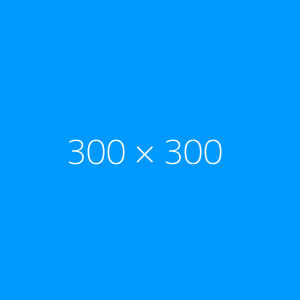
\includegraphics[width=1.0\textwidth,valign=t]{pictures/placeholder}
	\end{columns}
\end{frame}

\section{Installation}
\begin{frame}\frametitle{Installation}
	\begin{itemize}
		\item code und zeug
	\end{itemize}
\end{frame}

\section{"'Hello World"'-Beispiel}
\section{Grenzen von Hybrid-Apps}
\section{Sensorik-Nutzung}

\begin{frame}
	\centering
	\textcolor{cordovablue}{{\LARGE Vielen Dank für Ihre Aufmerksamkeit!\\[6ex] Fragen?}}
\end{frame}

\begin{frame}\frametitle{Quellen}
\begin{itemize}
	\item https://cordova.apache.org/
	\item https://ccoenraets.github.io/cordova-tutorial/index.html
\end{itemize}
\end{frame}

\end{document}